\chapter{Kimia Bioanorganik}\label{ch:b3:bioinorganic}

Darah kita merah karena besi; darah belangkas tidak berwarna di dalam
pembuluhnya dan menjadi biru di udara, karena darah itu membawa oksigen pada tembaga.
Kehidupan memakai segelintir ion logam untuk tugas-tugas yang tidak dapat dikerjakan gugus organik mana pun: mengikat
oksigen secara reversibel, memindahkan elektron satu per satu, memecah air, mereduksi nitrogen,
membuat molekul air cukup asam untuk menyerang karbon dioksida. Bab ini
membaca tugas-tugas itu dengan perangkat kimia koordinasi: \omterm{def:b3:bioinorganic:hsab}{asam keras} dan \omterm{def:b3:bioinorganic:hsab}{asam
lunak}, medan ligan dan keadaan spin, kesetimbangan dan hukum laju, dan bab ini ditutup
dengan logam-logam yang dipakai sebagai obat.

\begin{recall}
Jilid Tahun 2 membahas asam $\alpha$-amino, rantai samping dan peptida, basa nukleat
dan nukleotida, kompleks koordinasi, medan ligan, spin tinggi dan spin rendah, serta
nukleofil dan elektrofil keras dan lunak; Jilid Tahun 1 membahas tetapan
kompleksasi dan skala pL. \Cref{ch:b3:complex-spectra-magnetism} dan
\cref{ch:b3:complex-mechanisms} memberikan spektrum, teori Marcus, dan akuasi
cisplatin, \cref{ch:b3:complex-kinetics} kinetika Michaelis--Menten, dan
\cref{ch:b3:advanced-nmr} waktu relaksasi $T_1$.
\end{recall}

\begin{omfigure}
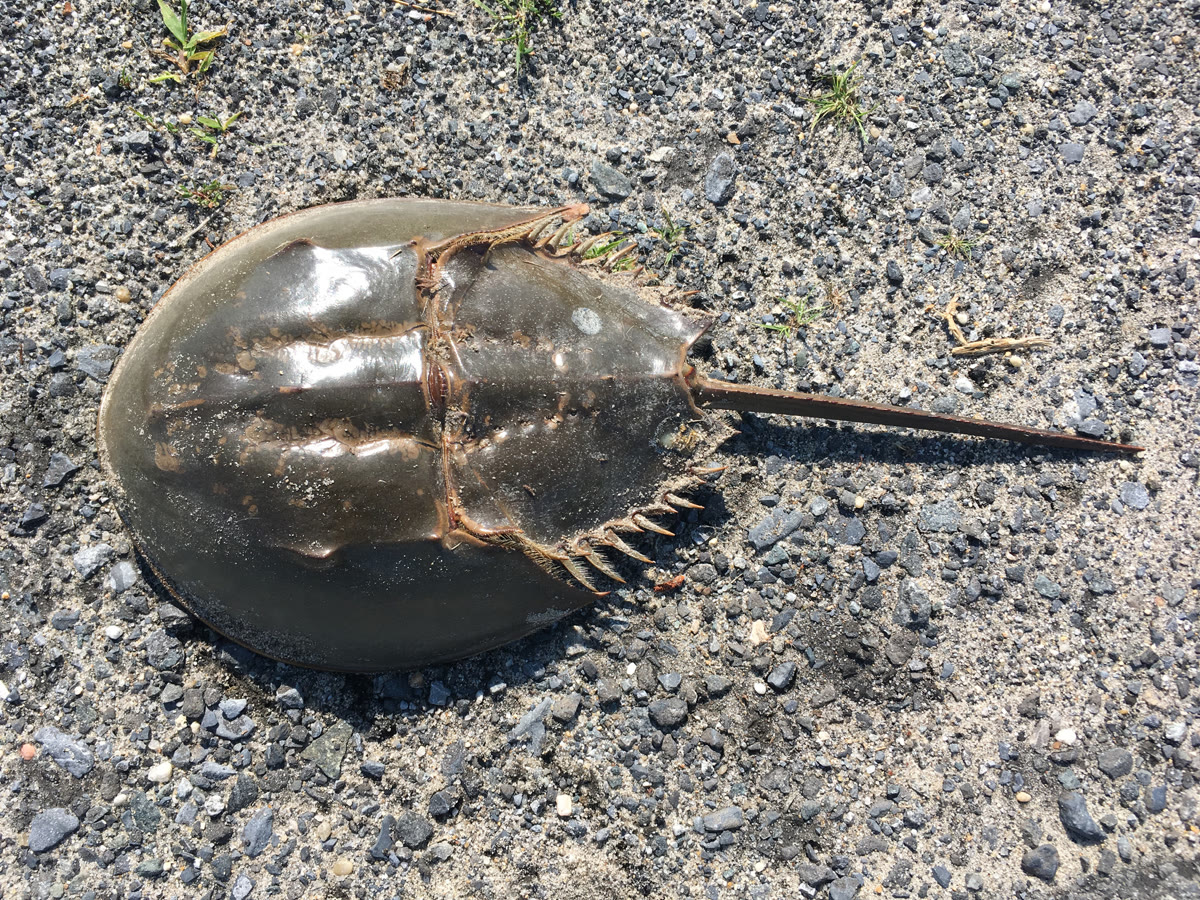
\includegraphics[width=0.5\linewidth]{images/book4/horseshoe-crab.jpg}

{\small Seekor belangkas Atlantik. Darahnya membawa oksigen pada hemosianin, sebuah
protein tembaga, dan berwarna biru ketika teroksigenasi. Foto: Kaldari, CC0.}
\end{omfigure}

\section{Logam dalam biologi}

\begin{definition}[Metaloprotein]\label{def:b3:bioinorganic:metalloprotein}
Yang disebut \emph{metaloprotein}\index{metaloprotein} adalah protein yang mengandung
ion logam terikat; \emph{metaloenzim}\index{metaloenzim} adalah metaloprotein yang
mengkatalisis sebuah reaksi. Yang disebut \emph{kofaktor}\index{kofaktor} adalah spesies nonprotein,
yaitu ion logam atau molekul kecil, yang terikat pada protein dan diperlukan untuk
aktivitasnya.
\end{definition}

Logam-logam yang penting dalam jumlah besar adalah natrium, kalium, magnesium, dan
kalsium, yang terutama membawa muatan dan menopang struktur; logam transisi
besi, seng, tembaga, mangan, kobalt, molibdenum, dan nikel terdapat dalam jumlah renik
tetapi menjalankan sebagian besar kimianya. Sebuah protein memilih logamnya melalui atom-atom donor
yang ditawarkannya beserta geometrinya.

\begin{definition}[Asam keras dan asam lunak]\label{def:b3:bioinorganic:hsab}
Yang disebut \emph{asam keras}\index{asam keras} adalah asam Lewis yang kecil, bermuatan tinggi, dan sukar
terpolarisasi ($\ce{H+}$, $\ce{Mg^2+}$, $\ce{Ca^2+}$, $\ce{Fe^3+}$); sedangkan \emph{asam
lunak}\index{asam lunak} adalah asam Lewis yang besar, mudah terpolarisasi, dan bermuatan rendah ($\ce{Cu+}$, $\ce{Ag+}$,
$\ce{Hg^2+}$, $\ce{Cd^2+}$). Menurut \emph{asas asam--basa keras dan lunak}\index{asas asam--basa keras dan lunak},
asam keras lebih suka terikat pada basa keras
(donor oksigen, fluorida) dan asam lunak pada basa lunak (donor belerang, iodida).
\end{definition}

Dalam protein, karboksilat dan fenolat bersifat keras, tiolat sisteina dan
tioeter metionina bersifat lunak, dan imidazol histidina berada di antaranya. Besi(III)
berada di antara donor-donor oksigen, tembaga(I) di antara donor-donor belerang, dan seng, asam
perbatasan, bersama histidina dan sisteina; raksa dan kadmium beracun sebagian
karena keduanya merebut sisteina-sisteina \omterm{def:b3:complex-kinetics:enzyme}{enzim}.

\begin{definition}[Deret Irving--Williams]\label{def:b3:bioinorganic:irving-williams}
Yang disebut \emph{deret Irving--Williams}\index{deret Irving--Williams} adalah urutan
kestabilan kompleks spin tinggi ion-ion divalen deret transisi
pertama dengan sebuah ligan tertentu:
$\ce{Mn^2+} < \ce{Fe^2+} < \ce{Co^2+} < \ce{Ni^2+} < \ce{Cu^2+} > \ce{Zn^2+}$.
\end{definition}

\begin{proposition}[Urutan Irving--Williams]\label{prop:b3:bioinorganic:irving-williams}
Deret itu berlaku untuk hampir semua ligan (sebuah pengamatan eksperimen); deret itu
mengikuti penurunan jari-jari ion dari mangan ke tembaga, energi stabilisasi medan
ligan, yang nol untuk $d^5$ dan terbesar untuk $d^8$, serta distorsi Jahn--Teller
tembaga(II), yang memperpendek empat ikatannya.
\end{proposition}

\begin{proof}[Argumen]
Jari-jari mengecil sepanjang baris ketika muatan inti bertambah, sehingga
tarikan elektrostatik setiap ligan menguat. Stabilisasi medan ligan
ion-ion oktahedral spin tinggi (\cref{ch:b3:complex-spectra-magnetism}) adalah $0$, $4$,
$8$, $12$, dan $6\,\mathrm{Dq}$ untuk $d^5$ sampai $d^9$, dan $0$ untuk $d^{10}$: stabilisasi itu menambah kecenderungan tersebut sampai nikel dan
anjlok untuk seng; tembaga(II) memperoleh kembali lebih banyak daripada yang ditunjukkan stabilisasinya melalui
distorsi tetragonalnya, yang memberikan empat ikatan pendek yang kuat.
\end{proof}

Sebuah akibat yang harus dikelola sel: tembaga dan seng akan mengalahkan
ion-ion lain di sebagian besar situs, sehingga konsentrasi bebasnya dijaga sangat rendah
oleh protein-protein pembawa khusus.

\section{Transpor oksigen}

\begin{definition}[Porfirin dan hem]\label{def:b3:bioinorganic:haem}
Yang disebut \emph{porfirin}\index{porfirin} adalah makrosiklus aromatik besar dan datar dari empat
cincin pirol yang dihubungkan oleh jembatan metina, yang keempat nitrogennya mengikat ion logam
di pusatnya. Yang disebut \emph{hem}\index{hem} adalah kompleks besi protoporfirin~IX,
yaitu \omterm{def:b3:bioinorganic:metalloprotein}{kofaktor} hemoglobin, mioglobin, dan sitokrom.
\end{definition}

Dalam mioglobin dan hemoglobin, besi \omterm{def:b3:bioinorganic:haem}{hem} memiliki ligan kelima di bawah
cincin, yaitu nitrogen histidina proksimal, dan situs keenam yang bebas untuk $\ce{O2}$.
Besi(II) deoksi berspin tinggi: elektron di orbital $d_{x^2-y^2}$, yang mengarah ke keempat
nitrogen, membuatnya terlalu besar untuk lubang cincin, sehingga besi itu berada di luar
bidang, ke arah histidina. Ketika mengikat $\ce{O2}$, besi itu menjadi berspin rendah, lebih kecil, dan
bergerak masuk ke dalam bidang, sambil menarik histidina dan heliks protein bersamanya.

\begin{omfigure}
% ledger: pdb:Hb.deoxy.FeN4, pdb:Hb.oxy.FeN4
\begin{tikzpicture}[font=\small, scale=0.9]
  \foreach \x/\lab/\dz/\oxy in {0/deoksi (spin tinggi)/-0.34/0, 6.4/oksi (spin rendah)/-0.04/1} {
    \begin{scope}[xshift=\x cm]
      \draw[omDef, line width=2.6pt] (-2.2,0) -- (2.2,0);
      \node[font=\scriptsize, anchor=west, omDef] at (2.3,0) {porfirin};
      \fill[omThm] (0,\dz*1.5) circle (0.22);
      \node[font=\scriptsize, anchor=north west] at (0.2,\dz*1.5-0.12) {Fe};
      \draw[black!70, line width=1pt] (0,\dz*1.5-0.22) -- (0,-1.55);
      \node[draw=black!70, regular polygon, regular polygon sides=5, minimum size=7mm, inner sep=0pt] at (0,-1.95) {};
      \node[font=\scriptsize, anchor=west] at (0.45,-1.95) {His proksimal};
      \node[font=\small\bfseries] at (0,1.9) {\lab};
      \ifnum\oxy=1
        \draw[black!70, line width=1pt] (0,0.2) -- (0,0.85) -- (0.55,1.25);
        \fill[red!75] (0,0.85) circle (0.13) (0.55,1.25) circle (0.13);
        \node[font=\scriptsize, anchor=west] at (0.75,1.2) {$\ce{O2}$, bengkok};
      \fi
    \end{scope}
  }
  \draw[<->, black!60] (-1.0,0) -- (-1.0,-0.51) node[midway, left, font=\scriptsize] {\qty{0.34}{\angstrom}};
\end{tikzpicture}

{\small Besi \omterm{def:b3:bioinorganic:haem}{hem} yang dilihat dari samping, dengan pergeserannya dari cincin digambar sesuai
skala (1~\AA{} sebagai 1.35~cm; jarak-jarak lainnya skematis). Dalam deoksihemoglobin, besi(II) berspin tinggi terletak
\qty{0.34}{\angstrom} di bawah bidang rata-rata keempat nitrogen pirol, di sisi
histidina proksimal; dalam oksihemoglobin, besi itu berada dalam jarak \qty{0.05}{\angstrom} dari bidang, dengan $\ce{O2}$
yang terikat melalui ujungnya dan bengkok (jarak dihitung dari struktur kristal).}
\end{omfigure}

Dioksigen yang terikat lebih tepat digambarkan sebagai superoksida pada besi(III), $\ce{Fe^{III}-O2^-}$, daripada
sebagai $\ce{O2}$ netral pada besi(II): kompleks itu diamagnetik karena elektron-elektron
tak berpasangan kedua pusat itu berkopling. Protein mencegah oksidasi
ireversibel menjadi besi(III) dan air, yang langsung dialami \omterm{def:b3:bioinorganic:haem}{hem} telanjang di dalam
air.

\begin{definition}[Pengikatan kooperatif]\label{def:b3:bioinorganic:cooperativity}
Pengikatan pada protein yang memiliki beberapa situs disebut \emph{kooperatif}\index{pengikatan kooperatif}
jika terikatnya satu ligan menaikkan afinitas situs-situs
yang tersisa. Yang disebut \emph{koefisien Hill}\index{koefisien Hill} $n$ adalah kemiringan
plot Hill, $\log\frac{\theta}{1 - \theta}$ terhadap $\log p$, pada setengah kejenuhan ($\theta$ adalah fraksi situs
yang terisi).
\end{definition}

\begin{proposition}[Satu situs]\label{prop:b3:bioinorganic:hyperbola}
Untuk protein dengan satu situs, $\mathrm{P + O_2 \rightleftharpoons PO_2}$, fraksi yang terisi adalah $\theta = p/(p_{50} + p)$, dengan $p_{50}$
tetapan disosiasi yang dinyatakan sebagai tekanan.
\end{proposition}

\begin{proof}
$K_d = [\mathrm P]p/[\mathrm{PO_2}] = p_{50}$, sehingga $[\mathrm{PO_2}] = [\mathrm P]p/p_{50}$, dan $\theta = [\mathrm{PO_2}]/([\mathrm P] + [\mathrm{PO_2}]) = (p/p_{50})/(1 + p/p_{50})$.
\end{proof}

\begin{theorem}[Persamaan Hill]\label{thm:b3:bioinorganic:hill}
Untuk protein dengan $n$ situs yang semuanya kosong atau semuanya terisi,
$\mathrm{P + n\,O_2 \rightleftharpoons P(O_2)_n}$,
\[
  \theta = \frac{p^n}{p_{50}^n + p^n}, \qquad \log\frac{\theta}{1 - \theta} = n\log p - n\log p_{50}.
\]
\end{theorem}

\begin{proof}
$K_d = [\mathrm P]p^n/[\mathrm{P(O_2)_n}]$; tuliskan $K_d = p_{50}^n$. Fraksi situs yang terisi sama dengan fraksi molekul
dalam bentuk terisi, $\theta = [\mathrm{P(O_2)_n}]/([\mathrm P] + [\mathrm{P(O_2)_n}]) = (p/p_{50})^n/(1 + (p/p_{50})^n)$. Maka $\theta/(1 - \theta) = (p/p_{50})^n$, dan dengan mengambil
logaritmanya diperoleh garis lurus dengan kemiringan $n$.
\end{proof}

Hemoglobin, dengan empat situs, tidak sepenuhnya \omterm{def:b3:bioinorganic:cooperativity}{kooperatif}: \omterm{def:b3:bioinorganic:cooperativity}{koefisien Hill-nya}
jauh di bawah 4, sekitar 3, dan plot Hill-nya berkemiringan 1 di kedua ujungnya, tempat
hemoglobin berperilaku sebagai protein deoksi atau protein oksi dengan situs-situs yang saling bebas.
Kooperativitas itu berasal dari perubahan struktur kuaterner: gerak
besi ke dalam bidang \omterm{def:b3:bioinorganic:haem}{hem} pertama yang mengikat $\ce{O2}$ diteruskan ke subunit-subunit lainnya.

\begin{omfigure}
\begin{tikzpicture}
\begin{axis}[name=a, width=0.48\linewidth, height=5.6cm, xmin=0, xmax=14, ymin=0, ymax=1.02,
  axis lines=left, xlabel={$p(\ce{O2})$ / \unit{kPa}}, ylabel={kejenuhan $\theta$},
  tick label style={font=\scriptsize}, label style={font=\small}]
\addplot[omMeth, thick] table[x=p, y=Mb] {figdata/out/bachelor-3-oxygen-binding.dat};
\addplot[omThm, thick] table[x=p, y=Hb] {figdata/out/bachelor-3-oxygen-binding.dat};
\addplot[omThm, thick, dashed] table[x=p, y=Hbacid] {figdata/out/bachelor-3-oxygen-binding.dat};
\draw[black!35] (axis cs:5,0) -- (axis cs:5,1.0) (axis cs:13,0) -- (axis cs:13,1.0);
\node[font=\scriptsize, anchor=south] at (axis cs:5,0.02) {jaringan};
\node[font=\scriptsize, anchor=south east] at (axis cs:13,0.02) {paru-paru};
\node[font=\scriptsize, omMeth] at (axis cs:1.9,0.96) {Mb};
\node[font=\scriptsize, omThm] at (axis cs:7.5,0.6) {Hb};
\end{axis}
\begin{axis}[at={(a.east)}, anchor=west, xshift=1.4cm, width=0.48\linewidth, height=5.6cm,
  xmin=-1.5, xmax=1.5, ymin=-3, ymax=3, axis lines=left,
  xlabel={$\log_{10}(p/\unit{kPa})$}, ylabel={$\log_{10}\bigl(\theta/(1-\theta)\bigr)$},
  tick label style={font=\scriptsize}, label style={font=\small}]
\draw[black!30] (axis cs:-1.5,0) -- (axis cs:1.5,0);
\addplot[omMeth, thick] table[x=lgp, y=Mb] {figdata/out/bachelor-3-oxygen-binding-b.dat};
\addplot[omThm, thick, restrict y to domain=-3:3] table[x=lgp, y=Hb] {figdata/out/bachelor-3-oxygen-binding-b.dat};
\node[font=\scriptsize, omMeth, anchor=west] at (axis cs:-1.1,1.4) {kemiringan 1};
\node[font=\scriptsize, omThm, anchor=east] at (axis cs:1.45,-1.5) {kemiringan 2.7};
\end{axis}
\end{tikzpicture}

{\small Kiri: kejenuhan oksigen mioglobin (hijau) dan hemoglobin (merah;
putus-putus: pada pH yang lebih rendah) terhadap tekanan oksigen, dengan nilai model
$p_{50} = \qty{0.37}{kPa}$ (Mb) dan \qty{3.5}{kPa} (Hb), $n = 2.7$. Antara paru-paru dan jaringan, hemoglobin
melepaskan seperempat oksigennya, mioglobin hampir tidak sama sekali. Kanan: plot
Hill yang bersesuaian, berupa garis lurus dalam model ini (plot hemoglobin yang sebenarnya
melengkung menjadi berkemiringan 1 di kedua ujungnya).}
\end{omfigure}

\begin{method}[Membaca plot Hill]\label{met:b3:bioinorganic:hill-plot}
\begin{enumerate}
  \item Dari setiap kejenuhan terukur, hitunglah $\log(\theta/(1 - \theta))$; alurkan nilai itu terhadap $\log p$.
  \item Tekanan tempat plot itu memotong nol adalah $p_{50}$.
  \item Kemiringan di titik itu adalah \omterm{def:b3:bioinorganic:cooperativity}{koefisien Hill}: $n = 1$ berarti situs-situs yang saling
        bebas, $n > 1$ \omterm{def:b3:bioinorganic:cooperativity}{pengikatan kooperatif}.
  \item Dengan dua titik saja, $n = \Delta\log(\theta/(1 - \theta))/\Delta\log p$.
\end{enumerate}
\end{method}

Hemoglobin juga mengikat proton dan karbon dioksida pada situs-situs yang jauh dari \omterm{def:b3:bioinorganic:haem}{hem},
yang menggeser kurvanya ke kanan di tempat keduanya melimpah, yaitu di jaringan yang sedang bekerja:
efek Bohr melepaskan lebih banyak oksigen tepat di tempat oksigen itu diperlukan.

\begin{proposition}[Persaingan karbon monoksida]\label{prop:b3:bioinorganic:haldane}
Jika karbon monoksida dan dioksigen bersaing memperebutkan situs yang sama, dengan
$\mathrm{HbO_2 + CO \rightleftharpoons HbCO + O_2}$ yang tetapan kesetimbangannya $M$, maka
$[\mathrm{HbCO}]/[\mathrm{HbO_2}] = M\,p(\ce{CO})/p(\ce{O2})$.
\end{proposition}

\begin{proof}
Pada kesetimbangan $M = [\mathrm{HbCO}]\,p(\ce{O2})/([\mathrm{HbO_2}]\,p(\ce{CO}))$; penyusunan ulang memberikan hasil itu.
\end{proof}

$M$ bernilai ratusan untuk hemoglobin manusia, sehingga beberapa ratus bagian per
juta karbon monoksida menempati sebagian besar situs; lebih buruk lagi,
situs-situs yang tersisa memegang oksigennya lebih erat, karena kooperativitas
bekerja pada situs-situs itu. \omterm{def:b3:bioinorganic:haem}{Hem} bebas mengikat karbon monoksida jauh lebih kuat lagi: dalam
protein, histidina distal di atas besi menghalangi geometri Fe--C--O linear
yang disukai karbon monoksida, sementara histidina itu membentuk ikatan hidrogen dengan $\ce{O2}$ yang bengkok.
Hewan-hewan lain memakai logam lain: hemosianin moluska dan artropoda
mengikat $\ce{O2}$ di antara dua ion tembaga sebagai peroksida, sedangkan hemeritrin beberapa cacing
laut mengikatnya pada sepasang ion besi.

\begin{inthelab}[Kurva pengikatan oksigen]
Larutan hemoglobin dalam bufer ditempatkan dalam kuvet kedap gas yang dilengkapi
labu samping. Larutan itu mula-mula dibebaskan dari oksigen dengan membilasnya dengan nitrogen, lalu
volume udara yang diketahui disuntikkan dan larutannya disetimbangkan dengan dimiringkan
perlahan-lahan. Setelah setiap penambahan, spektrum daerah tampak direkam: pita-pita
bentuk deoksi (satu pita di dekat \qty{555}{nm}) digantikan oleh dua pita bentuk oksi,
dan kejenuhannya dibaca dari absorbansi pada satu panjang gelombang, di antara batas
deoksi dan batas oksinya.
\end{inthelab}

\section{Metaloenzim}

Karbonat anhidrase mempercepat $\ce{CO2 + H2O <=> HCO3- + H+}$, yang dalam air saja memerlukan
beberapa detik, cukup lama untuk menjadi penting selama perjalanan singkat sel darah merah melalui kapiler
paru-paru. Ion sengnya dipegang oleh tiga histidina dan sebuah molekul air. Sebagai
kation kecil bermuatan tinggi, seng menurunkan $\mathrm pK_a$ air itu dari sekitar 14 menjadi
sekitar 7: pada pH fisiologis, sebagian besar \omterm{def:b3:complex-kinetics:enzyme}{enzim} membawa hidroksida yang terikat pada seng,
sebuah nukleofil kuat, yang dipegang tepat di samping kantong yang mengikat $\ce{CO2}$.

\begin{omfigure}
\begin{tikzpicture}[font=\small, >=Stealth]
  \node (a) at (90:2.0) {$\mathrm{(His)_3Zn{-}OH_2}$};
  \node (b) at (0:2.9) {$\mathrm{(His)_3Zn{-}OH^-}$};
  \node (c) at (-90:2.0) {$\mathrm{(His)_3Zn{-}OCO_2H^-}$};
  \draw[->, thick] (a) to[bend left=25] node[midway, above right, font=\scriptsize] {$-\,\ce{H+}$ (ke histidina pengantar)} (b);
  \draw[->, thick] (b) to[bend left=25] node[midway, below right, font=\scriptsize, align=left] {$+\,\ce{CO2}$:\\ serangan nukleofilik} (c);
  \draw[->, thick] (c) to[bend left=35] node[midway, left, font=\scriptsize, align=right] {$+\,\ce{H2O}$\\ $-\,\ce{HCO3-}$} (a);
\end{tikzpicture}

{\small Siklus katalitik karbonat anhidrase. Air yang terikat pada seng melepaskan sebuah
proton; hidroksida yang terikat pada seng menyerang karbon dioksida; air menggantikan
hidrogenkarbonat. Transfer proton ke pelarut adalah tahap yang paling lambat.}
\end{omfigure}

\begin{proposition}[Enzim yang cepat]\label{prop:b3:bioinorganic:carbonic-anhydrase}
\omterm{def:b3:complex-kinetics:michaelis}{Tetapan spesifisitas} $k_{\mathrm{cat}}/K_M$ karbonat anhidrase mendekati tetapan laju
pertemuan $\ce{CO2}$ dengan \omterm{def:b3:complex-kinetics:enzyme}{enzim}: hampir setiap pertemuan berujung pada
reaksi.
\end{proposition}

\begin{proof}[Argumen]
$k_{\mathrm{cat}}/K_M$ adalah tetapan laju orde dua \omterm{def:b3:complex-kinetics:enzyme}{enzim} dan substrat pada konsentrasi substrat yang rendah
(\cref{ch:b3:complex-kinetics}); nilainya tidak dapat melampaui
tetapan laju pertemuan keduanya yang \omterm{def:b3:rate-theories:diffusion}{dikendalikan difusi}
(\cref{ch:b3:rate-theories}). Nilai-nilai terukur untuk karbonat anhidrase termasuk
yang tertinggi yang dikenal untuk \omterm{def:b3:complex-kinetics:enzyme}{enzim} mana pun dan mendekati batas itu: kimia
di dalam \omterm{def:b3:complex-kinetics:enzyme}{situs aktif} dengan demikian bukan lagi pembatas lajunya.
\end{proof}

\omterm{def:b3:complex-kinetics:enzyme}{Enzim} sitokrom P450, di hati dan di banyak sel lain, menghidroksilasi ikatan
C--H obat dan hormon. Besi \omterm{def:b3:bioinorganic:haem}{hemnya} dipegang oleh tiolat sisteina; dengan
$\ce{O2}$ dan dua elektron, besi itu membentuk kompleks okso besi(IV) dengan sebuah radikal pada
\omterm{def:b3:bioinorganic:haem}{porfirin}, yang disebut senyawa I, yang mengambil sebuah atom hidrogen dari
substrat lalu mengembalikan gugus hidroksil ke radikal karbon itu. Nitrogenase
mereduksi $\ce{N2}$ menjadi amonia pada suhu kamar pada gugusan tujuh atom besi,
satu molibdenum, dan sembilan sulfida di sekitar sebuah atom karbon pusat, yaitu \omterm{def:b3:bioinorganic:metalloprotein}{kofaktor}
FeMo, dengan mengorbankan banyak molekul ATP. Vitamin $\mathrm{B_{12}}$ mengandung
ikatan kobalt--karbon, salah satu dari sedikit sekali ikatan logam--karbon dalam biologi, yang
homolisisnya memulai penataan ulang radikal.

\section{Transfer elektron dan energi}

Protein yang hanya memindahkan elektron memiliki pusat logam dengan \omterm{def:b3:complex-mechanisms:reorganisation}{energi
reorganisasi} yang kecil (\cref{ch:b3:complex-mechanisms}): kedua bilangan
oksidasinya memiliki geometri yang hampir sama, sehingga penghalang Marcus rendah.

\begin{definition}[Gugusan besi--belerang]\label{def:b3:bioinorganic:fes}
Yang disebut \emph{gugusan besi--belerang}\index{gugusan besi--belerang} adalah sekelompok ion
besi yang dijembatani oleh ion sulfida dan terikat pada protein oleh tiolat sisteina:
$\ce{[2Fe-2S]}$, $\ce{[3Fe-4S]}$, dan $\ce{[4Fe-4S]}$ yang mirip kubana.
\end{definition}

\begin{definition}[Protein tembaga biru]\label{def:b3:bioinorganic:blue-copper}
Yang disebut \emph{protein tembaga biru}\index{protein tembaga biru} adalah protein yang membawa satu
ion tembaga yang diikat oleh dua histidina, sebuah sisteina, dan sebuah metionina yang terikat lemah dalam
situs tetrahedral yang terdistorsi; warna birunya yang pekat berasal dari pita transfer muatan
sisteina-ke-tembaga(II).
\end{definition}

\begin{definition}[Keadaan entatik]\label{def:b3:bioinorganic:entatic}
Yang disebut \emph{keadaan entatik}\index{keadaan entatik} adalah situs logam yang dipegang oleh
protein dalam geometri yang tegang, di antara geometri-geometri yang disukai oleh kedua
bilangan oksidasinya, yang menurunkan \omterm{def:b3:complex-mechanisms:reorganisation}{energi reorganisasi} reaksi-reaksinya.
\end{definition}

Tembaga(II) sendirian menyukai bidang segi empat, tembaga(I) tetrahedron: dalam situs
tembaga biru, tidak satu pun terpuaskan, dan transfer elektron berlangsung cepat.

\begin{definition}[Kompleks pelepas oksigen]\label{def:b3:bioinorganic:oec}
Yang disebut \emph{kompleks pelepas oksigen}\index{kompleks pelepas oksigen}
fotosistem~II adalah gugusan $\mathrm{Mn_4CaO_5}$ yang mengoksidasi air menjadi dioksigen dalam
fotosintesis.
\end{definition}

\begin{proposition}[Empat foton per oksigen]\label{prop:b3:bioinorganic:kok}
Mengoksidasi dua molekul air menjadi satu $\ce{O2}$ memerlukan empat foton yang diserap oleh
fotosistem~II, sementara gugusan itu melewati lima keadaan $\mathrm S_0$ sampai $\mathrm S_4$.
\end{proposition}

\begin{proof}
$\ce{2H2O -> O2 + 4H+ + 4e-}$: empat elektron harus dilepaskan. Setiap foton yang diserap oleh
pusat reaksi memindahkan satu elektron menjauh darinya, dan gugusan itu mengisi kembali
pusat yang teroksidasi satu elektron demi satu: empat foton, empat tahap, yang menyimpan
ekuivalen pengoksidasi dalam keadaan $\mathrm S_1$ sampai $\mathrm S_4$; $\mathrm S_4$ melepaskan $\ce{O2}$ dan kembali ke $\mathrm S_0$.
\end{proof}

\begin{omfigure}
\begin{tikzpicture}[font=\small, >=Stealth]
  \foreach \i/\ang in {0/90, 1/18, 2/-54, 3/-126, 4/162} {
    \node[draw, circle, minimum size=9mm, fill=omDef!10] (s\i) at (\ang:2.0) {$\mathrm S_{\i}$};
  }
  \foreach \i/\j in {0/1, 1/2, 2/3, 3/4} {
    \draw[->, thick] (s\i) to[bend left=18] node[midway, sloped, above, font=\scriptsize] {$h\nu$, $-\mathrm e^-$} (s\j);
  }
  \draw[->, thick, omThm] (s4) to[bend left=18] node[midway, sloped, above, font=\scriptsize] {$-\ce{O2}$, $+\,\ce{2H2O}$} (s0);
\end{tikzpicture}

{\small Siklus Kok \omterm{def:b3:bioinorganic:oec}{kompleks pelepas oksigen}. Setiap foton yang diserap oleh
fotosistem~II melepaskan satu elektron dari gugusan mangan (proton-proton
pergi di sepanjang jalan); oksidasi keempat memberikan $\mathrm S_4$, yang melepaskan dioksigen dan
kembali mengikat dua molekul air.}
\end{omfigure}

Di ujung lain rantai energi, sitokrom $c$ oksidase
mitokondria mereduksi $\ce{O2}$ menjadi air dengan empat elektron dan empat proton pada
besi \omterm{def:b3:bioinorganic:haem}{hem} dan ion tembaga yang saling berhadapan, tanpa melepaskan superoksida atau peroksida,
yaitu bentuk yang tereduksi sebagian dan merusak.

\section{Logam dalam kedokteran}

\begin{definition}[Obat logam]\label{def:b3:bioinorganic:metallodrug}
Yang disebut \emph{obat logam}\index{obat logam} adalah obat yang aktivitasnya bergantung pada
ion logam atau kompleks logam.
\end{definition}

Cisplatin, \textit{cis}-$\ce{[PtCl2(NH3)2]}$, stabil di dalam darah, yang konsentrasi kloridanya
tinggi; di dalam sel, tempat konsentrasi itu jauh lebih rendah, cisplatin mempertukarkan satu klorida dengan air
(\cref{ch:b3:complex-mechanisms}). Kompleks akuanya mengikat atom N7
guanina, lalu guanina kedua di sebelahnya pada untai yang sama: ikatan silang 1,2-GG
itu membengkokkan DNA, yang tidak dapat diperbaiki sel, sehingga sel itu mati. Isomer
\textit{trans} tidak dapat menjembatani dua basa yang bertetangga dan tidak aktif.
Karboplatin, dengan dikarboksilat pengelat yang lepas dengan lambat, memiliki lebih sedikit
efek samping; oksaliplatin, dengan ligan diaminosikloheksana, bekerja pada tumor
yang resisten terhadap cisplatin.

\begin{omfigure}
\begin{tikzpicture}[font=\small]
  \draw[black!60, line width=1.4pt] (-3.2,0) -- (3.2,0);
  \node[font=\scriptsize, anchor=west] at (3.3,0) {untai DNA};
  \foreach \x/\b in {-2.4/C, -1.0/G, 1.0/G, 2.4/T} {
    \draw[black!60, line width=1pt] (\x,0) -- (\x,0.6);
    \node[draw=black!70, fill=white, rounded corners=1pt, minimum width=6mm] (n\b\x) at (\x,0.9) {\b};
  }
  \node (pt) at (0,2.4) {$\ce{Pt}$};
  \draw[omThm, thick] (pt) -- (-0.95,1.2) node[midway, left, font=\scriptsize] {N7};
  \draw[omThm, thick] (pt) -- (0.95,1.2) node[midway, right, font=\scriptsize] {N7};
  \draw (pt) -- (-0.5,3.1) node[above left, font=\scriptsize, inner sep=1pt] {$\ce{H3N}$};
  \draw (pt) -- (0.5,3.1) node[above right, font=\scriptsize, inner sep=1pt] {$\ce{NH3}$};
\end{tikzpicture}

{\small Ikatan silang 1,2 di dalam satu untai yang dibuat cisplatin, skematis: setelah
melepaskan kedua kloridanya, platina mengikat atom-atom N7 dua guanina yang bersebelahan
pada satu untai, sambil mempertahankan kedua ligan amin \textit{cis}-nya. Kompleks adisi yang sebenarnya
membengkokkan heliks ganda.}
\end{omfigure}

\begin{definition}[Zat kontras]\label{def:b3:bioinorganic:contrast}
Yang disebut \emph{zat kontras}\index{zat kontras} untuk pencitraan resonansi magnetik adalah
senyawa paramagnetik yang memperpendek waktu relaksasi proton-proton air di
sekitarnya. Yang disebut \emph{relaksivitas}\index{relaksivitas} $r_1$ zat itu adalah kenaikan
laju relaksasi $1/T_1$ per satuan konsentrasi zat itu.
\end{definition}

\begin{proposition}[Laju relaksasi]\label{prop:b3:bioinorganic:relaxivity}
Dengan zat berelaksivitas $r_1$ pada konsentrasi $c$, laju relaksasi proton
air adalah $1/T_1 = 1/T_{1,0} + r_1c$, dengan $T_{1,0}$ nilainya tanpa zat itu.
\end{proposition}

\begin{proof}
Kontribusi paramagnetiknya sebanding dengan jumlah molekul zat itu
yang dikunjungi molekul-molekul air per satuan waktu, jadi sebanding dengan $c$; laju relaksasi dari
mekanisme-mekanisme yang saling bebas saling menjumlah. Menurut definisi $r_1$, laju yang ditambahkan adalah $r_1c$.
\end{proof}

Gadolinium(III), $4f^7$ dengan tujuh elektron tak berpasangan dan spin elektron yang
berelaksasi lambat, adalah logam pilihan. $\ce{Gd^3+}$ bebas beracun: ion itu diberikan sebagai
kompleks yang sangat stabil dengan poliaminokarboksilat oktadentat yang menyisakan satu
situs untuk sebuah molekul air, yang bertukar cepat dengan air ruah dan meneruskan
relaksasi itu ke seluruh air.

\begin{definition}[Terapi kelasi]\label{def:b3:bioinorganic:chelation-therapy}
Yang disebut \emph{terapi kelasi}\index{terapi kelasi} adalah penyingkiran logam beracun
dari tubuh oleh ligan pengelat yang diberikan sebagai obat, yang membentuk kompleks stabil
dan larut yang kemudian diekskresikan.
\end{definition}

\begin{method}[Memilih obat pengelat]\label{met:b3:bioinorganic:choose-chelator}
\begin{enumerate}
  \item Bandingkan tetapan kestabilan pengelat itu dengan logam beracun
        dan dengan logam-logam esensial yang hadir dalam jumlah besar ($\ce{Ca^2+}$, $\ce{Mg^2+}$,
        $\ce{Zn^2+}$).
  \item Hitunglah kadar logam bebas $\mathrm{pM} = -\log[\mathrm M]$ yang disisakan pengelat itu pada
        konsentrasi dan pH tubuh: makin tinggi pM untuk logam beracun dan makin
        rendah pM untuk logam esensial, makin baik.
  \item Berikan pengelat yang sudah dimuati ion esensial pesaingnya (kompleks
        kalsium EDTA untuk timbal), sehingga pengelat itu bertukar alih-alih
        merampas kalsium dari darah.
  \item Periksalah kecocokan keras--lunak (donor belerang untuk raksa dan timbal, donor
        oksigen keras untuk besi(III)) dan bahwa kompleksnya diekskresikan.
\end{enumerate}
\end{method}

\begin{safety}{\ghs[0.62cm]{GHS05}\ghs[0.62cm]{GHS06}\ghs[0.62cm]{GHS08}}
% ledger: ghs4:cisplatin
Cisplatin: fatal jika tertelan, dapat menyebabkan kanker dan cacat genetik, dapat merusak
kesuburan, menyebabkan kerusakan mata yang serius dan reaksi alergi; zat itu hanya ditangani
sebagai larutan obat siap pakai, dengan sarung tangan, di dalam lemari berventilasi.
\end{safety}

\begin{history}[Sebuah struktur protein dan sebuah obat yang ditemukan secara kebetulan]
Max Perutz bekerja lebih dari dua puluh tahun untuk struktur sinar-X
hemoglobin, yang terpecahkan pada resolusi rendah pada 1959; bersama John Kendrew, yang memecahkan struktur
mioglobin, ia menerima Hadiah Nobel Kimia 1962. Pada 1965 Barnett
Rosenberg, yang mengalirkan arus di antara elektrode platina dalam biakan
bakteri, melihat bakteri itu tumbuh menjadi filamen panjang tanpa membelah; penyebabnya
bukan arus itu melainkan kompleks amin platina yang terbentuk dari elektrode. Kompleks itu
menjadi cisplatin, yang masih merupakan salah satu obat antikanker yang paling banyak dipakai.
\end{history}

\section{Latihan}

\begin{exercise}[$\star$]\label{exo:b3:bioinorganic:1}
Sebuah protein jenuh 20\,\% pada \qty{2.1}{kPa} oksigen dan 80\,\% pada \qty{5.9}{kPa}. Hitunglah
\omterm{def:b3:bioinorganic:cooperativity}{koefisien Hill-nya}.
\end{exercise}

\begin{exercise}[$\star$]\label{exo:b3:bioinorganic:2}
Urutkan $\ce{Zn^2+}$, $\ce{Mn^2+}$, $\ce{Cu^2+}$, $\ce{Fe^2+}$, $\ce{Ni^2+}$, dan $\ce{Co^2+}$ menurut kestabilan kompleksnya dengan
sebuah ligan tertentu, dan jelaskan tempat seng.
\end{exercise}

\begin{exercise}[$\star$]\label{exo:b3:bioinorganic:3}
Ramalkan donor protein yang disukai (karboksilat, tiolat sisteina,
imidazol histidina) oleh $\ce{Ca^2+}$, $\ce{Fe^3+}$, $\ce{Cu+}$, $\ce{Zn^2+}$, dan $\ce{Hg^2+}$.
\end{exercise}

\begin{exercise}[$\star$]\label{exo:b3:bioinorganic:4}
Berapa banyak elektron yang dilepaskan, dan berapa banyak foton yang diserap oleh fotosistem~II,
per molekul $\ce{O2}$ yang dilepaskan? Per mol?
\end{exercise}

\begin{exercise}[$\star\star$]\label{exo:b3:bioinorganic:5}
Dengan kurva model bab ini ($p_{50} = \qty{0.37}{kPa}$ untuk mioglobin; \qty{3.5}{kPa} dan $n = 2.7$ untuk
hemoglobin), hitunglah fraksi oksigen yang dilepaskan setiap protein antara
\qty{13}{kPa} (paru-paru) dan \qty{5}{kPa} (jaringan).
\end{exercise}

\begin{exercise}[$\star\star$]\label{exo:b3:bioinorganic:6}
Udara yang mengandung \qty{50}{ppm} karbon monoksida dihirup cukup lama sampai mencapai
kesetimbangan. Dengan $M = 230$ (data latihan) dan $p(\ce{O2})/p(\ce{CO})$ sama dengan nilai udara itu
(20.95\,\% oksigen), berapakah fraksi hemoglobin yang membawa CO?
\end{exercise}

\begin{exercise}[$\star\star$]\label{exo:b3:bioinorganic:7}
Berikan bilangan oksidasi formal ion-ion besi dalam gugusan $\ce{[Fe2S2(SR)4]^2-}$,
$\ce{[Fe2S2(SR)4]^3-}$, dan $\ce{[Fe4S4(SR)4]^2-}$ (SR: sisteinat, S: sulfida).
\end{exercise}

\begin{exercise}[$\star\star$]\label{exo:b3:bioinorganic:8}
Tuliskan akuasi pertama cisplatin, dan jelaskan mengapa akuasi itu lambat di dalam darah dan
lebih cepat di dalam sel. Atom DNA manakah yang diikat platina, dan mengapa isomer
\textit{trans} tidak aktif?
\end{exercise}

\begin{exercise}[$\star\star$]\label{exo:b3:bioinorganic:9}
Sebuah jaringan memiliki $T_1 = \qty{1.2}{s}$. Zat gadolinium dengan \omterm{def:b3:bioinorganic:contrast}{relaksivitas} $\qty{4.0}{L.mmol^{-1}.s^{-1}}$ mencapai \qty{0.10}{mmol/L}
di dalamnya (data latihan). Hitunglah $T_1$ yang baru.
\end{exercise}

\begin{exercise}[$\star\star\star$]\label{exo:b3:bioinorganic:10}
Sebuah pengelat L memiliki $\log K = 18.0$ dengan $\ce{Pb^2+}$ dan $10.7$ dengan $\ce{Ca^2+}$ (data latihan).
Hitunglah tetapan kesetimbangan $\ce{Pb^2+ + [CaL]^2- <=> [PbL]^2- + Ca^2+}$ dan jelaskan mengapa kompleks
kalsiumnya yang diberikan dan bukan ligan bebasnya.
\end{exercise}

\begin{exercise}[$\star\star\star$]\label{exo:b3:bioinorganic:11}
% ledger: enz:median.kcatKM
Karbonat anhidrase memiliki $k_{\mathrm{cat}}/K_M \approx \qty{1e8}{L.mol^{-1}.s^{-1}}$ (data latihan), sedangkan \omterm{def:b3:complex-kinetics:enzyme}{enzim} yang khas sekitar
$\qty{1e5}{L.mol^{-1}.s^{-1}}$. Pada $[\ce{CO2}] = \qty{1.0}{mmol/L}$, jauh di bawah $K_M$, bandingkan waktu yang diperlukan masing-masing untuk mengubah setengah
substrat dengan konsentrasi \omterm{def:b3:complex-kinetics:enzyme}{enzim} \qty{1.0}{\micro mol/L}.
\end{exercise}

\begin{exercise}[$\star\star\star$]\label{exo:b3:bioinorganic:12}
Dengan $M = 230$, tekanan karbon monoksida berapakah yang menempati setengah situs dengan
hadirnya udara bertekanan oksigen \qty{0.2095}{bar}? Nyatakan tekanan itu dalam ppm gas pada \qty{1}{bar}.
\end{exercise}

\section{Soal: Berapa Banyak Oksigen yang Diantarkan Darah?}

\begin{problem}[{Soal akhir pekan --- berapa banyak oksigen yang diantarkan darah? Kurva
Hill hemoglobin dan mioglobin, oksigen yang dibawa satu liter darah,
pergeseran Bohr, dan apa yang direnggut karbon monoksida}]
\label{pb:b3:bioinorganic:1}
% ledger: const:Vm1
Data model soal: hemoglobin $p_{50} = \qty{3.5}{kPa}$ dan $n = 2.7$ pada pH 7.4, $p_{50} = \qty{4.0}{kPa}$ pada
pH yang lebih rendah di jaringan yang sedang bekerja; mioglobin $p_{50} = \qty{0.37}{kPa}$; darah mengandung \qty{150}{g/L}
hemoglobin, dengan massa molar \qty{64.5}{kg/mol} dan empat situs per molekul; $p(\ce{O2})$ adalah \qty{13}{kPa}
di paru-paru dan \qty{5.0}{kPa} di jaringan; jantung memompa \qty{5.0}{L/min} saat istirahat;
$M = 230$ untuk karbon monoksida. Volume gas pada \qty{273.15}{K} dan \qty{101.325}{kPa}.

\medskip\noindent\textbf{Bagian I --- Kurva.}
\begin{enumerate}[beginpenalty=10000]
  \item Hitunglah kejenuhan hemoglobin di paru-paru.
  \item Hitunglah kejenuhan itu di jaringan pada pH 7.4.
  \item Hitunglah kejenuhan mioglobin pada \qty{5.0}{kPa}.
  \item Mengapa mioglobin dapat mengambil oksigen dari hemoglobin di dalam otot?
  \item \omterm{def:b3:bioinorganic:cooperativity}{Koefisien Hill} berapakah yang akan diberikan oleh empat situs yang saling bebas?
  \item Jelaskan dalam satu kalimat dari mana kooperativitas itu berasal.
\end{enumerate}

\medskip\noindent\textbf{Bagian II --- Satu liter darah.}
\begin{enumerate}[resume, beginpenalty=10000]
  \item Hitunglah konsentrasi hemoglobin dalam mol/L.
  \item Hitunglah konsentrasi situs oksigen.
  \item Hitunglah oksigen yang dibawa per liter di paru-paru, dalam mmol.
  \item Hitunglah oksigen yang diantarkan per liter ke jaringan pada pH 7.4.
  \item Konversikan nilai itu menjadi mililiter gas.
  \item Berapakah fraksi oksigen yang dibawa yang diwakili nilai itu?
\end{enumerate}

\medskip\noindent\textbf{Bagian III --- Pergeseran Bohr.}
\begin{enumerate}[resume, beginpenalty=10000]
  \item Hitunglah kejenuhan di jaringan pada pH yang lebih rendah.
  \item Hitunglah oksigen yang diantarkan per liter dengan pergeseran itu.
  \item Dengan faktor berapakah pergeseran itu menaikkan pengantaran?
  \item Apakah yang menurunkan pH otot yang sedang bekerja?
  \item Hitunglah oksigen yang diantarkan per menit saat istirahat, dalam mmol.
  \item Konversikan nilai itu menjadi liter gas per menit.
\end{enumerate}

\medskip\noindent\textbf{Bagian IV --- Karbon monoksida.}
\begin{enumerate}[resume, beginpenalty=10000]
  \item Hitunglah $[\mathrm{HbCO}]/[\mathrm{HbO_2}]$ untuk udara dengan \qty{100}{ppm} CO.
  \item Hitunglah fraksi situs yang hilang karena CO.
  \item Mengapa hilangnya oksigen yang diantarkan lebih buruk daripada fraksi itu?
  \item Mengapa oksigen murni merupakan penanganan pertama?
  \item Mengapa histidina distal penting bagi kelangsungan hidup?
  \item Nyatakan hasilnya: liter oksigen yang diantarkan per menit saat istirahat.
\end{enumerate}
\end{problem}
